\documentclass[10pt,a4paper]{article}
\usepackage[margin=22mm]{geometry}
\usepackage[T1]{fontenc}
\usepackage{lmodern,amsmath,amssymb,booktabs,graphicx,tikz,hyperref,fvextra}
\usetikzlibrary{arrows.meta,positioning,calc,decorations.pathmorphing}
\definecolor{ink}{RGB}{20,53,78}
\hypersetup{colorlinks=true,urlcolor=ink,linkcolor=ink}
\setlength{\parindent}{0pt}
\setlength{\parskip}{5pt}
\emergencystretch=3em

\title{\color{ink}Thermal enclosure and a slow sensor}
\author{}
\date{Original learning collection -- November 2026}
\begin{document}
\begin{center}{\LARGE\color{ink}Thermal enclosure and a slow sensor}\\[5pt]{\small Original learning collection -- November 2026}\end{center}

\textbf{Evidence note.} Original teaching scenario. Numerical parameters are deliberately chosen for learning. All generated data and curves are synthetic; no physical measurement is asserted.
\section{Design brief}
A camera enclosure receives a $40\,\mathrm{W}$ heat increment. Use thermal capacitance $C_{\mathrm{th}}=900\,\mathrm{J/K}$, conductance $H=15\,\mathrm{W/K}$ and sensor time constant $\tau_s=12\,\mathrm{s}$. Starting at ambient temperature, derive physical rise $x=T-T_a$ and sensor indication $y$, their poles and final values, and the sensor error after one enclosure time constant.
\section{Physical system}
\begin{center}\resizebox{\ifdim\width>.98\linewidth.98\linewidth\else\width\fi}{!}{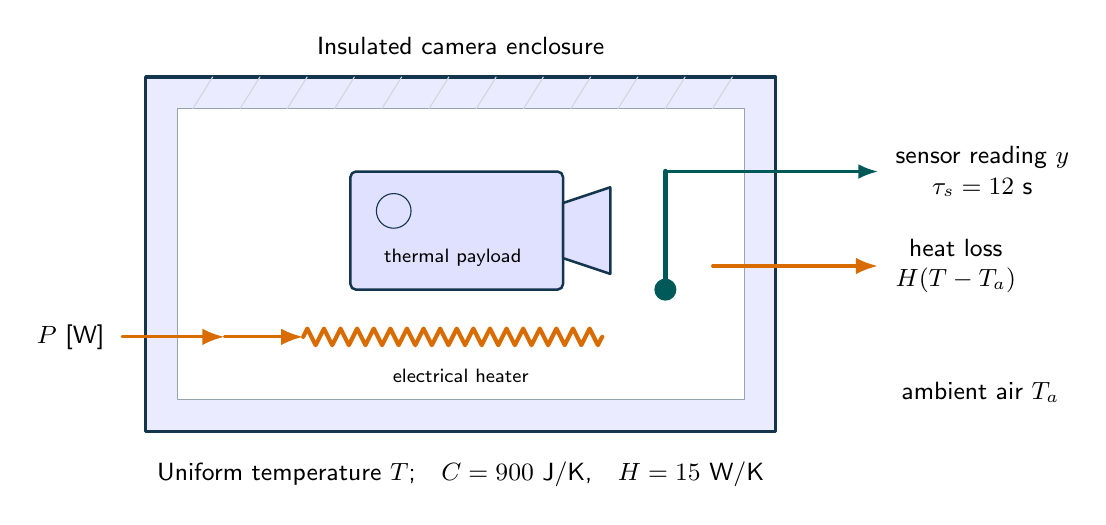
\begin{tikzpicture}[
font=\sffamily\small,>=Latex,line cap=round,line join=round,
wall/.style={draw=ink,line width=1.2pt,fill=blue!5},
water/.style={fill=cyan!25,draw=none},
metal/.style={draw=ink,fill=blue!12,line width=.9pt},
flow/.style={->,draw=blue!65!black,line width=1.2pt},
heat/.style={->,draw=orange!85!black,line width=1.1pt},
measure/.style={->,draw=teal!70!black,line width=.9pt},
dim/.style={<->,draw=ink!65,line width=.6pt},
spring/.style={draw=ink,decorate,decoration={coil,aspect=.5,segment length=4pt,amplitude=3pt}},
wire/.style={draw=ink,line width=1pt},
lab/.style={align=center,font=\sffamily\small},
smalllab/.style={align=center,font=\sffamily\scriptsize}]

\fill[blue!8] (1,0) rectangle (9,4.5);
\fill[white] (1.4,.4) rectangle (8.6,4.1);
\draw[ink,line width=1.2pt] (1,0) rectangle (9,4.5);
\draw[ink!45] (1.4,.4) rectangle (8.6,4.1);
\foreach \x in {1.6,2.2,...,8.2}{\draw[ink!20](\x,4.1)--++(.25,.4);}
\node[lab]at(5,4.9){Insulated camera enclosure};
\draw[metal,rounded corners=2pt](3.6,1.8)rectangle(6.3,3.3);
\draw[metal](6.3,2.2)--(6.9,2)--(6.9,3.1)--(6.3,2.9)--cycle;
\draw[ink](4.15,2.8)circle(.22);
\node[smalllab]at(4.9,2.2){thermal payload};
\draw[heat](2,1.2)--(3,1.2);
\draw[orange!85!black,line width=1.5pt,decorate,decoration={zigzag,segment length=6pt,amplitude=3pt}](3,1.2)--(6.8,1.2);
\node[lab,anchor=east]at(.6,1.2){$P$ [W]};
\draw[heat](.7,1.2)--(2,1.2);
\node[smalllab]at(5,.7){electrical heater};
\draw[teal!70!black,line width=2pt](7.6,1.8)--(7.6,3.3);
\fill[teal!70!black](7.6,1.8)circle(.14);
\draw[measure](7.6,3.3)--(10.3,3.3);
\node[lab,anchor=west]at(10.4,3.3){sensor reading $y$\\$\tau_s=12$ s};
\draw[heat](8.2,2.1)--(10.3,2.1);
\node[lab,anchor=west]at(10.4,2.1){heat loss\\$H(T-T_a)$};
\node[lab]at(11.6,.5){ambient air $T_a$};
\node[lab]at(5,-.55){Uniform temperature $T$;\quad $C=900$ J/K,\quad $H=15$ W/K};
\end{tikzpicture}
}\par{\small Cutaway of a lumped thermal enclosure. Orange arrows carry heat; the probe measures a lagged temperature. The drawing fixes the energy boundary, not a real device geometry.}\end{center}
\section{Energy balance}
Let $x=T-T_a$ denote temperature rise in kelvin and $P$ the incremental heat input in watts. With constant ambient temperature and a spatially uniform enclosure,
\[C_{th}\dot x=P-Hx,\qquad \tau_s\dot y=x-y.\]
The enclosure time constant is $\tau=C_{th}/H=60$ s and its static gain is $1/H=1/15$ K/W. The sensor does not change the enclosure energy balance.
\section{Cascade model}
Taking Laplace transforms with zero initial deviations gives
\[G_x(s)=\frac{1/15}{60s+1},\qquad G_y(s)=\frac{1/15}{(60s+1)(12s+1)}.\]
The physical and measured responses share the final rise $40/15=8/3$ K, but the measured path adds the pole $-1/12$ to the thermal pole $-1/60$.
\section{Closed-form step responses}
Integrating the energy balance gives $x(t)=\frac83(1-e^{-t/60})$. Partial fractions of $G_y(s)40/s$ give
\[y(t)=\frac83\left[1-\frac{60e^{-t/60}-12e^{-t/12}}{48}\right].\]
Both start at zero; $\dot x(0)=40/900$ K/s while $\dot y(0)=0$. Evaluate these expressions at $t=60$ s rather than treating 63.2 percent of the measured final value as the enclosure time constant.
\section{Model boundaries}
Heat leakage is linearized and the enclosure is assumed well mixed. Radiation, internal temperature gradients, sensor self-heating and changing ambient temperature are omitted. Every curve is a simulation with invented design parameters.
\section{What to learn from the experiment}
A slow sensor can hide a thermal excursion even when its final calibration is exact. Compare physical and measured states before estimating a time constant.
\section{System sketch}
\begin{center}\resizebox{\ifdim\width>.98\linewidth.98\linewidth\else\width\fi}{!}{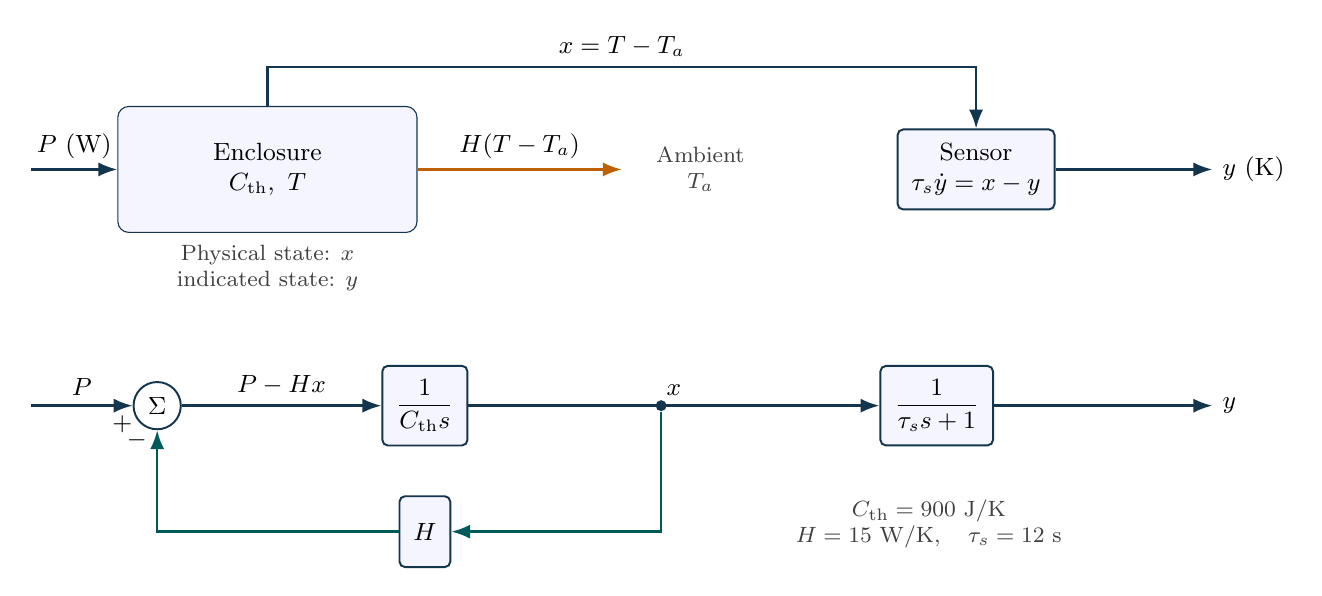
\begin{tikzpicture}[x=1cm,y=1cm,>=Latex,font=\small,
block/.style={draw=ink,fill=blue!4,rounded corners=2pt,minimum height=9mm,align=center,line width=.7pt,inner sep=5pt},
sum/.style={circle,draw=ink,fill=white,minimum size=6mm,inner sep=0pt,line width=.7pt},
sig/.style={->,draw=ink,line width=.85pt},
fb/.style={->,draw=teal!70!black,line width=.85pt},
dist/.style={->,draw=orange!75!black,line width=.85pt},
tap/.style={circle,fill=ink,inner sep=1.4pt},
note/.style={font=\footnotesize,align=center,text=black!75}]

\node[draw=ink,fill=blue!4,rounded corners,minimum width=38mm,minimum height=16mm,align=center](en)at(3,2.5){Enclosure\\$C_{\mathrm{th}},\ T$};
\draw[sig](0,2.5)--node[above]{$P$ (W)}(en.west);
\draw[dist](en.east)--node[above]{$H(T-T_a)$}(7.5,2.5);
\node[note]at(8.5,2.5){Ambient\\$T_a$};
\node[block](sensor)at(12,2.5){Sensor\\$\tau_s\dot y=x-y$};
\draw[sig](en.north)--(3,3.8)--node[above]{$x=T-T_a$}(12,3.8)--(sensor.north);
\draw[sig](sensor.east)--(15,2.5)node[right]{$y$ (K)};
\node[note]at(3,1.25){Physical state: $x$\\indicated state: $y$};
\node[sum](s)at(1.6,-.5){$\Sigma$};
\node[block](int)at(5,-.5){$\dfrac{1}{C_{\mathrm{th}}s}$};
\node[tap](xt)at(8,-.5){};
\node[block](gs)at(11.5,-.5){$\dfrac{1}{\tau_s s+1}$};
\draw[sig](0,-.5)--node[above]{$P$}node[pos=.9,below]{$+$}(s);
\draw[sig](s)--node[above]{$P-Hx$}(int);
\draw[sig](int)--node[above]{$x$}(gs);
\draw[sig](gs)--(15,-.5)node[right]{$y$};
\node[block](h)at(5,-2.1){$H$};
\draw[fb](xt)--(8,-2.1)--(h);
\draw[fb](h)--(1.6,-2.1)--node[pos=.9,left]{$-$}(s);
\node[note]at(11.4,-2){$C_{\mathrm{th}}=900\ \mathrm{J/K}$\\$H=15\ \mathrm{W/K},\quad\tau_s=12\ \mathrm{s}$};

\end{tikzpicture}
}
\par\small\refstepcounter{figure}\label{fig:system}\textbf{Figure \thefigure.} Thermal storage, heat leakage and sensor dynamics are separate elements. The lower loop implements the energy balance, not an added temperature controller.\end{center}
\section{Executed computational evidence}
\VerbatimInput[fontsize=\small,breaklines=true]{results.txt}
\begin{center}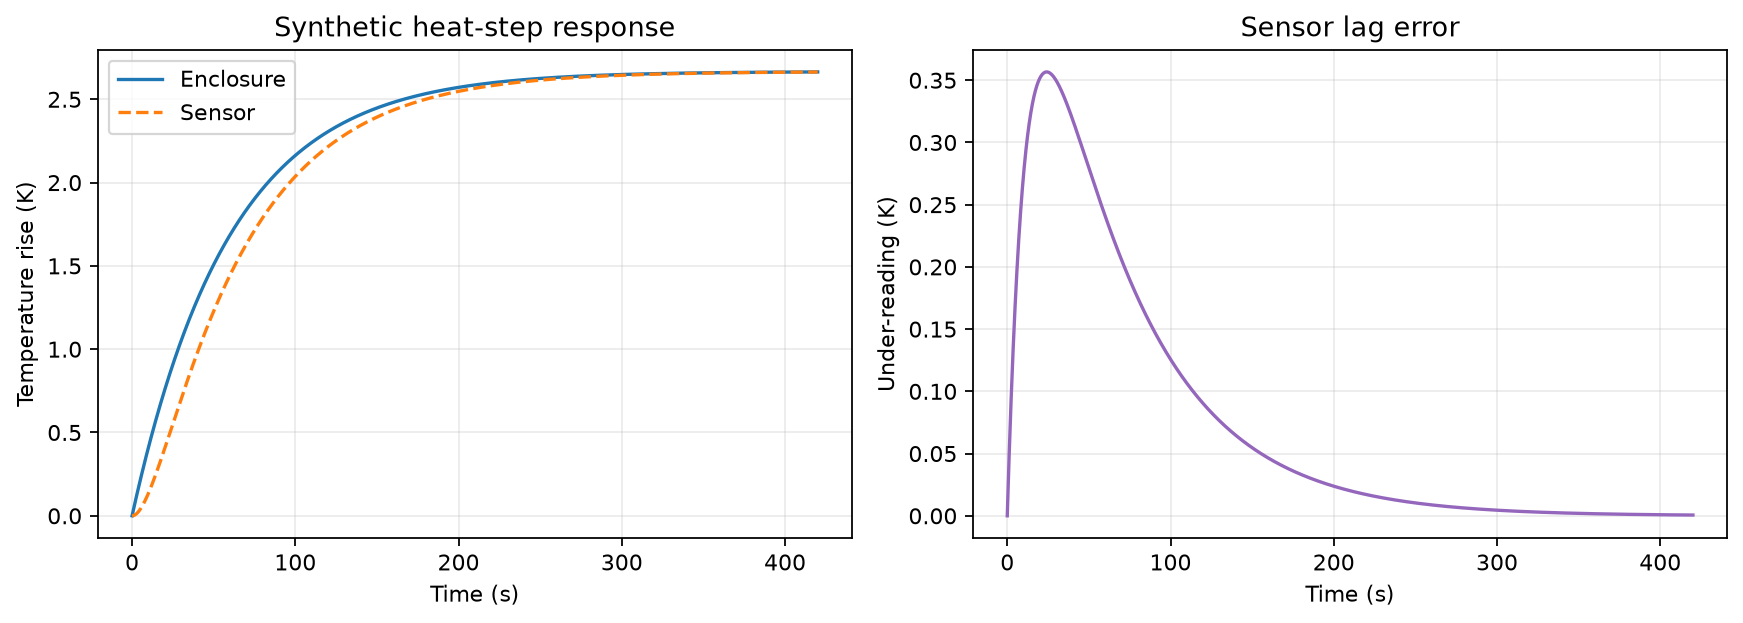
\includegraphics[width=\linewidth,height=.46\textheight,keepaspectratio]{response.png}\end{center}
\section{Method references}
The equations use standard balance laws and feedback-control methods. Further explanation: \url{https://apmonitor.com/pdc/} and \url{https://fbsbook.org/}. Implementation documentation: \url{https://python-control.readthedocs.io/en/0.10.2/}. See the repository reference catalog for individual topics and videos.
\end{document}
